\chapter{Einleitung}



\section{Motivation} \label{sec:Einl:Motivation}


Die von Hubkolbenmotoren beim Verbrennungsvorgang in den Zylindern erzeugten Kräfte und Momente 
verursachen Torsionsschwingungen der Kurbelwelle \cite{Denman:Tautochronic}.
Es existieren viele Methoden, wie beispielsweise der Einsatz von
Schwungrädern oder von abgestimmten Vibrationsdämpfern, zur Reduktion dieser Schwingungen \cite{ALSUWAIYAN:2002:PerformanceAnd}.
Schwungräder erhöhen jedoch  die Massenträgheit des Systems, was das Ansprechverhalten verschlechtert,
und Torsionsdämpfer dissipieren mechanische Energie und Arbeit 
nur bei genau einer Frequenz (oder in einem kleinen Frequenzbereich)
\cite{ALSUWAIYAN:2002:PerformanceAnd}.
Eine weitere effektive Methode zur Schwingungsreduktion ist der Einsatz von
Fliehkraftpendeln (engl. \new{centrifugal pendulum vibration absorber}, CPVA).
Dabei handelt es sich um passive Bauteile für den Einsatz bei rotierenden Maschinen oder
Hubkolbenmaschinen, um die dort auftretenden Torsionsschwingungen zu vermindern \cite{monroe2011accounting}.
Die ersten Patente für Fliehkraftpendel gehen auf den Zeitraum um 1930 zurück
\cite{Sarazin:1931:Patent}. 
Die zugrunde liegende, lineare Theorie ist beispielsweise in 
\cite{Desoyer-Slibar:1953:BerechnungVonPendelTilgern,  Paslay:Slibar:1956:OptAusSalomonTilger, 
Schick:1939:WirkungFliehkraftpendel, Slibar-Desoyer:1954:ZurErzielungOptimaler}
dargestellt.
Die damals entwickelten Fliehkraftpendel wurden zunächst hauptsächlich in Flugzeugen eingesetzt, um die
Torsionsschwingungen der Rotoren, welche mit fast konstanter Drehzahl $\Omega$ betrieben wurden,
zu reduzieren \cite{Vidmar:Feeney:2012:CoulombFriction}. 

Im Laufe der Zeit fanden die Fliehkraftpendel auch Anwendung im Automobilbereich,
wobei sich hier $\Omega$ über einen großen Betriebsbereich erstreckt 
\cite{Vidmar:Feeney:2012:CoulombFriction}.
Das im Hubkolbenmotor beim Verbrennungsvorgang erzeugte Moment $M$, welches die Welle zu Torsionsschwingungen anregt, 
kann durch eine harmonische Anregung $M=M_0 \cos(k_E \Omega t)$ modelliert werden \cite{Denman:Tautochronic},
wobei $k_E \Omega$ die Frequenz des anregenden Moments, $k_E$ die  Anregungsordnung und $M_0$ die 
Amplitude des anregenden Moments beschreibt. 
Die Anregungsordnung  $k_E$ ist dabei direkt von der Zylinderzahl $N$ des Verbrennungsmotors,
welcher die  rotierende Welle antreibt,  abhängig
und für  Viertaktmotoren gilt $k_E=\nicefrac{N}{2}$ \cite{Denman:Tautochronic}.
Beispielsweise besitzt ein Viertaktmotor mit drei Zylindern die Anregungsordnung $k_E = \nicefrac{3}{2}$. 

Die ersten Fliehkraftpendel zur Schwingungsreduktion wurden als einfache Pendel realisiert, 
welche über eine Aufhängung an der rotierenden Welle 
befestigt und so ausgelegt wurden, dass die Eigenfrequenz bzw. Periode des Pendels
mit der Anregungsfrequenz bzw. Periode des externen, anregenden Moments übereinstimmt \cite{Denman:Tautochronic}.
%
%
\begin{figure}[ht]%
	\centering
	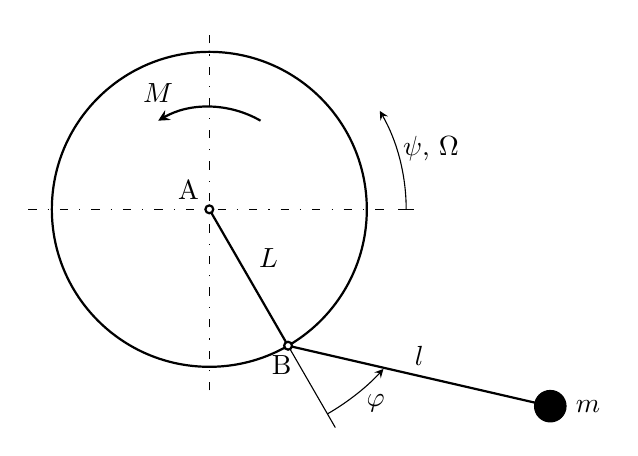
\begin{tikzpicture}[>=stealth]
\draw [loosely dashdotted] (-2.3,0) -- (2.3,0);
\draw [loosely dashdotted](0,-2.3) -- (0,2.3);
\draw [thick] (0,0) circle (2cm);


\draw [thick] (0mm,0mm) -- node[anchor=south west]{$L$} (-60:2);
%\draw (0,0) -- (-60:3);
%\draw [->] (-60:2.8cm) arc (-45:2.8cm:2.8cm);

\draw [->, thick] (60:1.3cm) arc (60:120:1.3cm) node[above=0.1cm]{$M$};

% Bemaßung Omega
\draw [->] (0:2.5cm) arc (0:30:2.5cm) node[right=0.65cm,below=0.2cm]{$\psi$, $\Omega$};
\draw  (2.4,0) -- (2.6,0);

% Bemaßung l und m
\draw  [thick] (-60:2) -- node[anchor=south]{$l$} (-30:5);
\filldraw (-30:5) circle (.2cm) node[right=0.2cm]{$m$};

% Bemaßung Winkel
\draw (-60:2) --  (-60:3.2);
\draw [->] (-60:3cm) arc (-60:-42.5:3cm) node[left=0.1cm, below=0.2cm]{$\varphi$};


% Einfügen der Punkte A und B
\filldraw[fill=white, draw=black, thick] (0,0) circle (0.05cm) node[anchor=south east]{A};
\filldraw[fill=white, draw=black, thick] (-60:2) circle (0.05cm) node[left=0.08cm,below]{B};
\end{tikzpicture}

%	\includegraphics{Grafiken/GEinleitung/Punktmasse.pdf}
	\caption{Prinzipskizze eines einfachen Fliehkraftpendels}
	\label{fig:Einleitung:PendelMitPunktmasse}
\end{figure}
%
%
Wie exemplarisch in \figref{fig:Einleitung:PendelMitPunktmasse} dargestellt ist, bewegt  sich dabei ein solches
Pendel (Masse $m$) auf einer Kreisbahn um einen festen Aufhängepunkt am Rotor \cite{Denman:Tautochronic}.
 \figref{fig:Einleitung:PendelMitPunktmasse} zeigt eine um den Punkt A
 mit Drehzahl $\Omega$ rotierende Welle (Rotor) im Querschnitt.
Mit $\psi$ wird der Verdrehwinkel des Rotors bezeichnet, welcher sich bei konstanter
Rotordrehzahl $\Omega$ zu $\psi = \Omega t$ ergibt.
Im Abstand $L$ vom Mittelpunkt A ist im Aufhängepunkt B die Punktmasse $m$ über einen
idealisiert masselosen Stab der Länge $l$  befestigt.
Die Auslenkung von $m$ relativ zur rotierenden Welle wird mit $\varphi$ bezeichnet.
%
%
%
Durch linearisierte Behandlung des als Punktmasse idealisierten Fliehkraftpendels
nach \figref{fig:Einleitung:PendelMitPunktmasse} resultiert als
Differentialgleichung für kleine Winkel $\varphi$
\begin{equation}
	ml\ddot{\varphi} + m L \Omega^2 \varphi = 0.
\label{eq:Einleitung:DGLLinearisiertesSystem}
\end{equation}
%
%
Die Eigenkreisfrequenz des Fliehkraftpendels ist 
\begin{equation}
	\omega_{F} = \Omega \sqrt{\frac{L}{l}} = k \Omega,
\label{eq:Einleitung:EigenfrequenzFliehkraftpendel}
\end{equation}
welche direkt proportional zur Wellendrehzahl $\Omega$ ist und vom geometrischen Faktor $k=\sqrt{\frac{L}{l}}$,
welcher hier als \new{lineares Tuning}, \new{lineare Tuningordnung} oder \new{lineare Abstimmungsordnung}  
bezeichnet wird, abhängt \cite{Schick:1939:WirkungFliehkraftpendel}.
Das Fliehkraftpendel tilgt die durch Erregung der
Ordnung $k_E$ hervorgerufenen Drehschwingungen, wenn
seine Eigenkreisfrequenz $\omega_{F}$ gleich der Anregungsfrequenz $k_E \Omega$ 
ist \cite{Markert:2010:Fahrzeugschwingung, Schick:1939:WirkungFliehkraftpendel}.
Aus der linearen Theorie resultiert  als Abstimmungsbedingung somit die Relation
%
% 
%
\begin{equation}
	k = k_E,
\label{eq:Einleitung:LineareAbstimmungFliehkraftpendel}
\end{equation}
welche zur Erzielung günstiger Tilgerwirkung einzuhalten ist 
\cite{Schick:1939:WirkungFliehkraftpendel,  Slibar-Desoyer:1954:ZurErzielungOptimaler}.
Für die Wahl $k=k_E$ oszilliert die Pendelmasse in solch einer Art und Weise, 
dass die durch die Masse aufgrund der Fliehkraft erzeugte Momentenwirkung auf die Welle
dem anregenden Moment der Ordnung $k_E$ genau entgegenwirkt
\cite{Desoyer-Slibar:1953:BerechnungVonPendelTilgern,  Paslay:Slibar:1956:OptAusSalomonTilger, 
Schick:1939:WirkungFliehkraftpendel, Slibar-Desoyer:1954:ZurErzielungOptimaler}.
Die Wirkungsweise eines so ausgelegten Fliehkraftpendels ähnelt der eines abgestimmten, translatorischen
Schwingungstilgers  \cite{Vidmar:Feeney:2012:CoulombFriction}. 
Ein besonderer Vorteil eines solchen Fliehkraftpendels ist 
die Unabhängigkeit von der Rotordrehzahl $\Omega$ und somit von der Anregungsfrequenz
bei fester Anregungsordnung $k_E$, welche für einen Verbrennungsmotor in Abhängigkeit der Zylinderzahl konstant ist 
\cite{Schick:1939:WirkungFliehkraftpendel}. 
Damit ist das Pendel in beliebigen Betriebszuständen $\Omega \neq \const$ wirksam und
nicht nur bei einer bestimmten, konstanten Solldrehzahl  $\Omega$
bzw. konstanten Anregungsfrequenz $k_E \Omega$ \cite{Schick:1939:WirkungFliehkraftpendel}. 
%bzw. dem Prinzip zweier über eine Drehfeder mit Drehfedersteifigkeit $k_D$ gekoppelten Massenträgheiten $J_1$ und $J_2$.
%
%
%
Die Wirksamkeit solcher Absorber, bei denen sich die Pendelmasse auf einem Kreispfad bewegt (Kreisbahnpendel),
beschränkt sich allerdings auf den Bereich kleiner Pendelausschläge 
(kleine Winkel $\varphi$ in \figref{fig:Einleitung:PendelMitPunktmasse}).
Nichtlineare Effekte führen jedoch dazu, dass die Absorberfrequenz für große Absorberamplituden von
dieser Amplitude (Größe des Ausschlags von $\varphi$) abhängt \cite{LeeShaw:OnTheCounteraction}, was zur Folge
hat, dass die Wirkungsweise solch einfacher Absorber eingeschränkt ist \cite{ALSUWAIYAN:2002:PerformanceAnd}.
In der praktischen Umsetzung werden Kreisbahnpendel als Zweifadenpendel bzw. Pendel 
mit Doppelaufhängung (Doppelfadenpendel) realisiert \cite{Markert:2010:Fahrzeugschwingung}.


Die Periode eines einfachen Kreisbahnpendels ist bei niedrigen Pendelamplituden unabhängig von der Amplitude 
und wenn das Pendel richtig abgestimmt ist, also die richtige Eigenfrequenz besitzt, 
stellt diese Frequenz auch für größere Absorberamplituden (welche durch
größere Amplituden des anregenden Moments entstehen) die richtige Abstimmung dar.
Dies ist für solche Kreisbahnpendel gültig, bis nichtlineare Effekte, welche zur Änderung der Eigenfrequenz des Pendels führen,
signifikant werden \cite{Denman:Tautochronic, Haddow:2003:ExperimentalInv}.
Bei entsprechenden Werten der Anregungsamplitude vergrößert sich die Absorberperiode
des Kreisbahnpendels auf entsprechend große Werte, dass die lineare Theorie das Verhalten nicht mehr hinreichend
genau beschreibt, was zu einer erhöhten Drehmomentbelastung der Kurbelwelle führt
und bis hin zur Zerstörung führen kann \cite{Denman:Tautochronic}.
Dieser Effekt kann durch bewusstes \new{Mistuning}, 
d.\,h. der beabsichtigten Wahl von  $k \neq k_E$, abgemildert werden  \cite{ALSUWAIYAN:2002:PerformanceAnd}.
Um aber dem eben beschriebenen Verhalten möglichst vollständig vorzubeugen, werden Fliehkraftpendel so 
ausgelegt, dass ihre Periode unabhängig von der Amplitude des anregenden Moments und somit
unabhängig von der Absorberamplitude konstant bleibt \cite{Denman:Tautochronic}.
Durch die Wahl anderer Absorberpfade als eine Kreisbahn kann dies  auch für große 
Amplituden erreicht werden \cite{ALSUWAIYAN:2002:PerformanceAnd}. 
Dazu ist die bislang beschriebene kreisförmige Bahn für die Absorbermasse nicht mehr geeignet  \cite{Denman:Tautochronic}.

Wird die Pendelmasse durch vorgegebene Konturen auf Zykloiden oder Epizykloiden geführt,
können die eben beschriebenen Probleme bei Kreisbahnpendeln vermieden werden 
\cite{Denman:Tautochronic, Lee:TorsionalVibRed}. 
Die praktische Realisierung solcher Pfade ist in 
\cite{Denman:Tautochronic, Mayet:Experimental} dargestellt.
Durch Wahl einer besonderen Epizykloide, der Tautochrone, kann erreicht werden, 
dass die Absorberfrequenz für konstante Rotordrehzahl unabhängig von der Absorberamplitude 
bleibt \cite{Denman:Tautochronic}.
Die Eigenschaften eines tautochronen Absorber wurden eingehend in \cite{Denman:Tautochronic}
untersucht und bieten bedeutende Verbesserungen gegenüber Absorbern, welche sich
auf Kreisbahnen bewegen \cite{Denman:Tautochronic, LeeShaw:OnTheCounteraction}.
In \cite{Denman:Tautochronic} wurden die Absorber allerdings weiterhin als einfache
Punktmassen betrachtet.



Am Lehrstuhl für Angewandte Mechanik an der Technischen Universität München werden
Fliehkraftpendel zur passiven Schwingungsreduktion im Automobilbereich entwickelt.
Vor Kurzem wurden dabei gewonnene Forschungsergebnisse in einem Paper mit Titel
"`Tautochronic Centrifugal Pendulum Vibration Absorbers -- General Design and Analysis"' 
\cite{Mayet:Tautochronic} veröffentlicht. 
Dabei werden die Pendelmassen im Gegensatz zum in \cite{Denman:Tautochronic}
dargestellten tautochronen Entwurf von Fliehkraftpendeln nicht mehr als einfache 
Punktmassen betrachtet. 
Deshalb kann die Absorberdynamik nicht mehr durch die reine Bewegung des Pendelschwerpunkts
beschrieben werden, weshalb die in \cite{Denman:Tautochronic} hergeleiteten geometrischen
Beziehungen nicht mehr verwendet werden können \cite{Mayet:Tautochronic}.
Bei der in \cite{Mayet:Tautochronic} dargestellten Formulierung wird eine Rotation der
Pendel zugelassen und die Wirkung
der Massenträgheiten der Pendel mit in den tautochronen Entwurfsprozess aufgenommen.
Des Weiteren wird ein allgemeiner Ansatz für den tautochronen Absorberentwurf 
vorgeschlagen. 
Diese entwickelte \new{Guideline} erlaubt den einheitlichen Umgang mit einer Vielzahl
von verschiedenen Realisierungen von Fliehkraftpendeln und erweitert 
die bislang verwendeten Entwurfsverfahren \cite{Mayet:Tautochronic}.









%Bis ungefähr 1980 wurden diese einfachen, kreisförmigen Pfade zur Abstimmung der Fliehkraftpendel verwendet \cite{Mayet:Tautochronic}.























\section{Ziel der Arbeit}
%
% Optimales Tuning
In dem in  \cite{Mayet:Tautochronic} vorgeschlagenen Entwurfsformalismus ist keine
Dämpfung berücksichtigt. 
Bei der erweiterten Untersuchung eines auf Grundlage dieser Guideline entworfenen, tautochronen 
Fliehkraftpendels im weiteren Verlauf des Papers wird zusätzlich linear viskose Dämpfung
angesetzt, welche die Systemdynamik beeinflusst.
Die Wirkung des Fliehkraftpendels wird dabei auf Basis von Averaging-Gleichungen
untersucht, welche eine Approximation der stationären Systemantwort  darstellen.
Die Schwingungsreduktionswirkung des entworfenen Absorbers
mit linearem Tuning $k=k_E$ ist durch den Einfluss von viskoser Dämpfung 
bei der Anregungsordnung $k_E$ nicht optimal.
Das Fliehkraftpendel zeigt nicht bei der Anregungsordnung $k_E$ beste Wirkung,
sondern der Punkt bester Absorberwirkung verschiebt sich zu einer 
anderen Anregungsordnung $k_{E,shift}$. 
Je größer die  Dämpfung ist, desto ausgeprägter ist dieser Effekt.
Durch die freie Wahl des Absorbertunings $k$ wird eine Veränderung der Geometrie und somit
eine Veränderung der Dynamik bei weiterhin tautochronem Verhalten erreicht und es kann
dem ungewünschten Einfluss der viskosen Dämpfung entgegengewirkt werden. 
Im Rahmen dieser Arbeit soll das optimale Tuning $k$ eines Fliehkraftpendels
in Abhängigkeit linear viskoser Dämpfung allgemein bestimmt werden.
Besonders im Fokus steht dabei die Herleitung einer  analytischen Bedingung,
mit welcher das optimale Tuning $k$ bestimmt und somit
direkt im Entwurfsprozess berücksichtigt werden kann.

% Rotationsgradient
Durch die in \cite{Mayet:Tautochronic} dargestellte Formulierung kann der
Einfluss von  Rotation eines
Fliehkraftpendels und die Wirkung
der Massenträgheit des Pendels mit in den tautochronen Entwurfsprozess aufgenommen werden.
Die Auslegung eines solchen Rotationspendels wird in \cite{Mayet:Tautochronic} anhand
eines Beispiels veranschaulicht.
Dabei bleibt bei der Wahl des Rotationsgradienten, mit welchem die Absorberwirkung maßgeblich
beeinflusst werden kann, ein Term frei. Dieser Term ist vom Anwender zum Einstellen 
einer gewünschten Pendelwirkung zu wählen, wobei eine beliebige Wahl das tautochrone Verhalten
nicht beeinflusst, jedoch die resultierende Absorberwirkung verändert werden kann.
Dieser Term wird in \cite{Mayet:Tautochronic}  als konstant vorgeschlagen.
Eines der Hauptziele dieser Arbeit ist zu untersuchen, wie ein durch bestimmte Wahl des freien
Terms verallgemeinerter Rotationsgradient das Systemverhalten beeinflusst.
Insbesondere sollen dabei Aussagen zur Optimierung der Pendelwirkung durch
spezielle Wahl des Rotationsgradienten getroffen werden. 

% Nichtlineares Mistuning
Des Weiteren ist bekannt, dass die Absorberwirkung durch nichtlineares Mistuning 
erheblich beeinflusst werden kann \cite{Mayet:CPVAMitMistuning}. 
In \cite{Mayet:CPVAMitMistuning} wird ein Ansatz für das nichtlineare Mistuning vorgeschlagen,
welcher direkt in die Guideline aus \cite{Mayet:Tautochronic} aufgenommen werden kann,
jedoch noch nicht im Detail untersucht wurde.
Im Rahmen dieser Arbeit soll der Einfluss von nichtlinearem Mistuning nach dem 
in \cite{Mayet:CPVAMitMistuning} vorgeschlagenen Ansatz auf das Systemverhalten analysiert werden.
Dabei stehen zunächst qualitative Aussagen im Vordergrund. Allerdings sollen
aus den dadurch gewonnenen Erkenntnissen Vorschläge zur gezielten Beeinflussung
des Verhaltens der Fliehkraftpendel unter Berücksichtigung von nichtlinearem Mistuning
abgeleitet werden.




% Lösen der Averaging-Gleichung mit Bogenlängenverfahren
Um die bislang beschriebenen Hauptziele erreichen zu können, müssen die
in  \cite{Mayet:Tautochronic} hergeleiteten, nichtlinearen Averaging-Gleichungen gelöst werden.
Bei den numerischen Untersuchungen in \cite{Mayet:Tautochronic} wurden
die Averaging-Gleichungen, welche eine Approximation der stationären Systemantwort 
darstellen, für Spezialfälle gelöst.
Um dies aber auch für allgemeinere Fälle zu ermöglichen, muss die Lösung
der Averaging-Gleichungen mit einer Methode erfolgen, welche eine systematische Berechnung 
der stationären Systemantwort für alle Arten von Fliehkraftpendeln erlaubt.
Ein hierfür geeignetes Verfahren ist das Bogenlängenverfahren, welches im
Rahmen dieser Arbeit auf die Averaging-Gleichungen angewendet werden soll.
%Die damit erzielten Ergebnisse ermöglichen es, Aussagen über das stationäre
%Systemverhalten zu treffen  und können für den systematischen Auslegungsprozess
%von Fliehkraftpendeln genutzt werden.

% Vollständige Simulation der Bewegungsgleichungen
Um die Aussagekraft der auf Basis der Averaging-Gleichungen hergeleiteten Zusammenhänge
beurteilen zu können, sollen diese Ergebnisse durch die  Simulation der 
vollständigen, nicht vereinfachten, nichtlinearen Bewegungsgleichungen des
dynamischen Fliehkraftpendelsystems verifiziert werden. 
Dazu müssen die vollständigen Bewegungsgleichungen auf eine Art und Weise implementiert werden,
dass die erhaltenen Simulationsergebnisse direkt mit den 
Resultaten aus den Averaging-Gleichungen verglichen werden können.


% Zusammenfassender Satz
Im Rahmen dieser Arbeit soll auf Basis der Averaging-Gleichungen, deren
Aussagekraft durch anschließende Simulation der vollständigen, nichtlinearen Bewegungsgleichungen
beurteilt wird, das optimale lineare Tuning $k$ bestimmt,
der Einfluss eines verallgemeinerten Rotationsgradienten und die Berücksichtigung von 
nichtlinearem Mistuning auf das Systemverhalten untersucht werden. 









\section{Gliederung der Arbeit}


% Theorieteil, Kapitel 2
In \chref{ch:StandDerForschung} werden die theoretischen Grundlagen auf Basis der kürzlich
veröffentlichten Forschungsergebnisse \cite{Mayet:Tautochronic}, 
worauf in  dieser Arbeit aufgebaut wird, dargestellt.
Hierzu wird in \secref{sec:TautochronerEntwurfAllgemein} die entwickelte Formulierung
für den tautochronen Absorberentwurf dargelegt. 
Die Veranschaulichung der Sachverhalte, welche für diese Arbeit
grundlegend sind und auf welchen im weiteren Verlauf aufgebaut wird bzw.
worauf sich an späterer Stelle wieder bezogen wird, steht dabei im Vordergrund.
Es wird ein Einblick auf den grundlegenden Hintergrund dieser Arbeit gegeben.
Weiterführende Herleitungen und detaillierte Informationen können \cite{Mayet:Tautochronic} entnommen werde.
Anschließend wird in \secref{sec:TheorieMistuning} der in \cite{Mayet:CPVAMitMistuning} vorgeschlagene
Mistuning-Ansatz eingeführt. Dabei werden die Auswirkungen durch Berücksichtigung von nichtlinearem
Mistuning auf den in \cite{Mayet:Tautochronic} gegebenen Formalismus aufgezeigt.


% Vollständige Simulation
Um die Aussagekraft der auf Basis der Averaging-Gleichungen hergeleiteten Zusammenhänge
beurteilen zu können, wird  in \chref{cha:VollstaendigSimulation}
auf die Simulation der  vollständigen, nichtlinearen Bewegungsgleichungen 
von Fliehkraftpendelsystemen eingegangen.
Hierfür wird in \secref{sec:BewegungsgleichungenInMatlab} der strukturelle Aufbau der Bewegungsgleichungen 
nach dem Lagrange-Formalismus hergeleitet und
alle benötigten Terme explizit ermittelt, um ein vollständig bestimmtes Differentialgleichungssystem 
zur Implementierung zu erhalten.
Anschließend  wird auf Details und Besonderheiten bei der Implementierung 
in \textsc{Matlab} eingegangen (\secref{sec:ImplementierungInMatlab}).
Im Vordergrund steht dabei, dass die aus der Simulation des nichtlinearen Differentialgleichungssystems 
resultierenden Größen direkt mit den aus den Averaging-Gleichungen 
bestimmten Ergebnissen verglichen werden können. 
Dieses Kapitel wird dem darauffolgenden \chref{cha:LoesenAverGl} zur Lösung der Averaging-Gleichungen vorangestellt,
da zur vollständigen Bestimmung des Differentialgleichungssystems Ausdrücke hergeleitet werden,
welche im Anschluss bei der Lösung der Averaging-Gleichungen wiederverwendet werden können.


% Bogenlängenverfahren
Zur systematischen Lösung der Averaging-Gleichungen wird in \chref{cha:LoesenAverGl} das
Bogenlängenverfahren verwendet.
Zunächst wird  in  \secref{sec:Bogenlangenverfahren} der Grundgedanke des Verfahrens dargelegt 
und es werden grundlegende Vorteile des Verfahrens aufgezeigt. 
Bei der Herleitung wird die ursprüngliche, strukturmechanisch geprägte Terminologie verwendet und anschließend
auf die in den Averaging-Gleichungen auftretenden Größen übertragen.
Das Prinzip zur Lösung  der Averaging-Gleichungen wird  am 
Beispiel eines Absorbers demonstriert (\secref{sec:Bogenlaenge:UebertrafAufAveragingGleichungen}).
In \secref{sec:Bogenlange:Implementierung} wird auf  die praktische Umsetzung des Bogenlängenverfahrens eingegangen
und die Implementierung des Verfahrens in \textsc{Matlab} veranschaulicht.


% Optimales Tuning
Auf die allgemeine  Bestimmung des optimalen Tunings $k$ eines Fliehkraftpendels
in Abhängigkeit linear viskoser Dämpfung wird in \chref{cha:Optimierung} eingegangen.
Dabei wird zunächst in \secref{sec:Opt:SuboptDurchDaempfung}  aufgezeigt, wie die
Berücksichtigung von Dämpfung das Systemverhalten beeinflusst, wodurch
die Absorberperformance bei der Anregungsordnung $k_E$ nicht optimal ist.
Durch entsprechende Wahl des Absorbertunings kann die
bestmögliche Absorberwirkung dennoch bei der gewünschten Anregungsordnung erreicht werden.
Wie das Tuning explizit zu wählen ist, wird in  \secref{sec:Opt:BedingungFuerMinimum} veranschaulicht.
Anschließend wird in  \secref{sec:Opt:Bsp}
die Anwendung der hergeleiteten Zusammenhänge an einem Beispiel demonstriert.


% Untersuchung Rotationsgradient
In \chref{cha:EinflussRotGrad} wird der Einfluss eines verallgemeinerten
Rotationsgradienten auf das Systemverhalten untersucht.
Zunächst wird in \secref{sec:RotGrad:Ansatz} der verallgemeinerte Ansatz vorgestellt
und es werden die Auswirkungen auf andere funktionale Zusammenhänge im Entwurfsprozess dargelegt.
In \secref{sec:RotGrad:EinflussEinzelneTerme} wird der Einfluss dieses Ansatzes 
auf das Systemverhalten untersucht und anschließend wird in \secref{sec:UntersVariabRotGrad:GezielteMinimierung}
aufgezeigt, wie das Verhalten durch spezielle Wahl des Rotationsgradienten gezielt beeinflusst werden kann. 
Die durch die Averaging-Gleichungen prognostizierten Verbesserungen der Absorberperfor\-mance werden
in \secref{sec:RotGrad:VergleichSimulation} mit der vollständigen Simulation verglichen. 
%Da es hier zu deutlichen Abweichung kommt, scheinen die Averaging-Gleichung das Systemverhalten
%unter den dort getroffenen Annahmen nicht sonderlich gut zu approximieren.
In \secref{sec:RotGrad:BeruecksichtungTermeHoehererOrdnung} wird durch die Verwendung von 
Ansätzen höherer Ordnung die Approximation durch die Averaging-Gleichungen verbessert und aus den
daraus resultierenden Ergebnissen eine Aussage über das
optimale Verhalten eines Rotationspendels  getroffen.


% Untersuchung Mistuning
Die in \chref{cha:UntersuchungenMistuning} durchgeführten Untersuchungen zum Einfluss von nichtlinearem
Mistuning auf Basis der Averaging-Gleichungen  werden anhand eines Absorbers unter Verwendung
der Ergebnisse aus \chref{cha:EinflussRotGrad} demonstriert.
Dabei wird in \secref{sec:UntersMist:AnsatzMistuning} der verwendete Ansatz für das
nichtlineare Mistuning $u(s)$ vorgestellt und in \secref{sec:UntersMist:EinflussAufAverGl} der Einfluss dieses Ansatzes 
auf das Systemverhalten untersucht. Es wird aufgezeigt, wie das stationäre Verhalten des 
zugrunde liegenden Systems gezielt beeinflusst werden kann.
Die auf Basis der Averaging-Gleichungen prognostizierte Verbesserung der Fliehkraftpendelwirkung wird
in \secref{sec:Mistuning:AblgeichVollStSimul} mit der vollständigen Simulation verglichen.
%, wobei äußerste gute Übereinstimmung resultiert.
%
Daraus werden anschließend Folgerungen für den Absorberentwurf unter Berücksichtigung von
nichtlinearem Mistuning getroffen und
abschließend in \secref{sec:UntersMist:Einsatzmoeglichkeiten} exemplarisch aufgezeigt,
wie das Systemverhalten gezielt durch den Einsatz von nichtlinearem Mistuning beeinflusst werden kann.



% Schluss
\chref{cha:Schluss} fasst die wichtigsten Aspekte dieser Arbeit zusammen und gewährt einen Ausblick
auf Anwendungen und mögliche Erweiterungen.

















%\section{Tests}



%Textwidth: \the\textwidth 


%action-angle-Variablen: \cite{markus:1974:generic}

%und hier noch der Hagedorn \cite{Hagedorn:NichtlinSchwingungen1978}






%%%%%%%%%%%%%%%%%%%%%%%%%%%%%%%%%%%%%%%%%%%%%%%%%%%%%%%%%%%%%%%%%%%%%%%%%
% ZUNÄCHST ANGEDACHTE ERLÄUTERUNGEN
%%%%%%%%%%%%%%%%%%%%%%%%%%%%%%%%%%%%%%%%%%%%%%%%%%%%%%%%%%%%%%%%%%%%%%%%%



%
%Zwei Massen verbunden mit Feder (einfachst möglicher Fall, um Prinzip zu skizzieren):
%
%Periodische Anregung: 
%\begin{equation}
	%F(t) = F_0 \sin \left( \Omega t \right)
%\label{eq:PeriodischAnregendeKraft}
%\end{equation}
%
%%
%%
%%
%Bewegungsgleichungen:
%% 
%\begin{subequations}
	%\begin{align}
		%m_1 \ddot{x}_1 & = -k_{F} \left( x_1 - x_2 \right) + F_0 \sin \left( \Omega t \right) \\
		%m_2 \ddot{x}_2 & = k_{F} \left( x_1 - x_2 \right)
	%\end{align}
	%\label{eq:BewegungsleichungenTranslatorischerSchwingungstilger}	
%\end{subequations}
%
%%\begin{figure}[ht]
	%%\centering
	%%\def\svgwidth{0.3\textwidth}
	%%\import{./Grafiken/Zeichnung2/}{Versuch3.pdf_tex}
	%%\caption{Prinzipskizze eines Schwingungstilgers (translatorisch)}
%%\end{figure}
%
%
%Für stationäre Lösungen der fremderregten Schwingung resultiert mit
%\begin{equation}
		%x_1 = \hat{x}_{1} \sin \left( \Omega t \right), \qquad x_2 = \hat{x}_{2} \sin \left( \Omega t \right) 
	%\label{eq:BewegungsleichungenTranslatorischerSchwingungstilgerLoesungsansatz}	
%\end{equation}
%
%für die Amplitude $\hat{x}_{1}$ (hier noch ein Zitat hin)
%\begin{equation}
		%\hat{x}_{1} = \frac{F_0  \left(k_{F} - m_2 \Omega^2\right) }{m_1 m_2 \Omega^2 \left[ \Omega^2 - k_{F} \left(\frac{1}{m_1} + \frac{1}{m_2} \right) \right]} 
	%\label{eq:AmplitudeTranslatorischerSchwingungstilger}	
%\end{equation}
%
%
%Der prinzipielle Verlauf von $\hat{x}_{1}$ über $\Omega$ ist in (xxx) dargestellt. 
%
%%\begin{figure}[ht]
	%%\centering
	%%\def\svgwidth{\textwidth}
	%%\import{./Grafiken/Zeichnung2/}{Test1.pdf_tex}
	%%\caption{Amplitudenverlauf über $\Omega$}
%%\end{figure}
%
%
%
%
%
%
%
%%\begin{figure}[ht]
	%%\centering
	%%\def\svgwidth{0.5\textwidth}
	%%\import{./Grafiken/Zeichnung2/}{Drehfeder1.pdf_tex}
	%%\caption{Prinzipskizze eines Schwingungstilgers (translatorisch)}
%%\end{figure}
%
%
%
%%
%%
%%%%%%%%%%%%%%%%%%%%%%%%%%%%%%%%%%%%%%%%%%%%%
%% jetzt Torsionsschwinungen
%%%%%%%%%%%%%%%%%%%%%%%%%%%%%%%%%%%%%%%%%%%%%
%%
%%
%\newcommand{\WinkelA}{\beta}
%analog kann dies für Torsionsschwingungen hergeleitet werden \cite[Anhang A]{Denman:Tautochronic}, wobei Massen durch Massenträgheitsmomente, translatorische Freiheitsgrad durch rotatorische Freiheitsgrade und die Federsteifigkeit durch eine Drehfedersteifigkeit ersetzt werden, womit sich die folgenden Bewegungsgleichungen ergeben
%%
%%
%% Bewegungsgleichungen
%%
%\begin{subequations}
	%\begin{align}
		%\Theta_1 \ddot{\WinkelA}_1 & = -k_{D} \left( \WinkelA_1 - \WinkelA_2 \right) + M_0 \sin \left( \Omega t \right) \\
		%\Theta_2 \ddot{\WinkelA}_2 & = k_{D} \left( \WinkelA_1 - \WinkelA_2 \right)
	%\end{align}
	%\label{eq:BewegungsleichungenLinearerTorsionsschwingungsAbsorber}%	
%\end{subequations}
%%
%%
%und für die stationäre Lösung mit Ansatz  $\WinkelA_1 = \hat{\WinkelA}_{1} \sin \left( \Omega t \right)$, $\WinkelA_2 = \hat{\WinkelA}_{2} \sin \left( \Omega t \right)$ sich der Amplitudenverlauf
%%
%%
%%
%\begin{equation}
		%\hat{\WinkelA}_{1} = \frac{M_0  \left(k_{D} - \Theta_2 \Omega^2\right) }{\Theta_1\Theta_2 \Omega^2 \left[ \Omega^2 - k_{D} \left(\frac{1}{\Theta_1} + \frac{1}{\Theta_2} \right) \right]} 
	%\label{eq:AmplitudeRotatorischerSchwingungstilger}	
%\end{equation}
%und somit die Resonanzkurve analog ergibt. Anhand von Gleichung 	\eqref{eq:AmplitudeRotatorischerSchwingungstilger}	 ist klar ersichtlich, dass die Amplitude für
%%
%%
%% Verschwinden der Amplitude
%%
%\begin{equation}
		%k_{D} = \Theta_2 \Omega^2
	%\label{eq:AmplitudeRotatorischerSchwingungstilgerBedinungungfuerVerschwinden}	
%\end{equation}
%verschwindet



